\begin{wrapfigure}{r}{0.525\textwidth} 
	\vspace{-.75em}
	\begin{center}
		\fbox{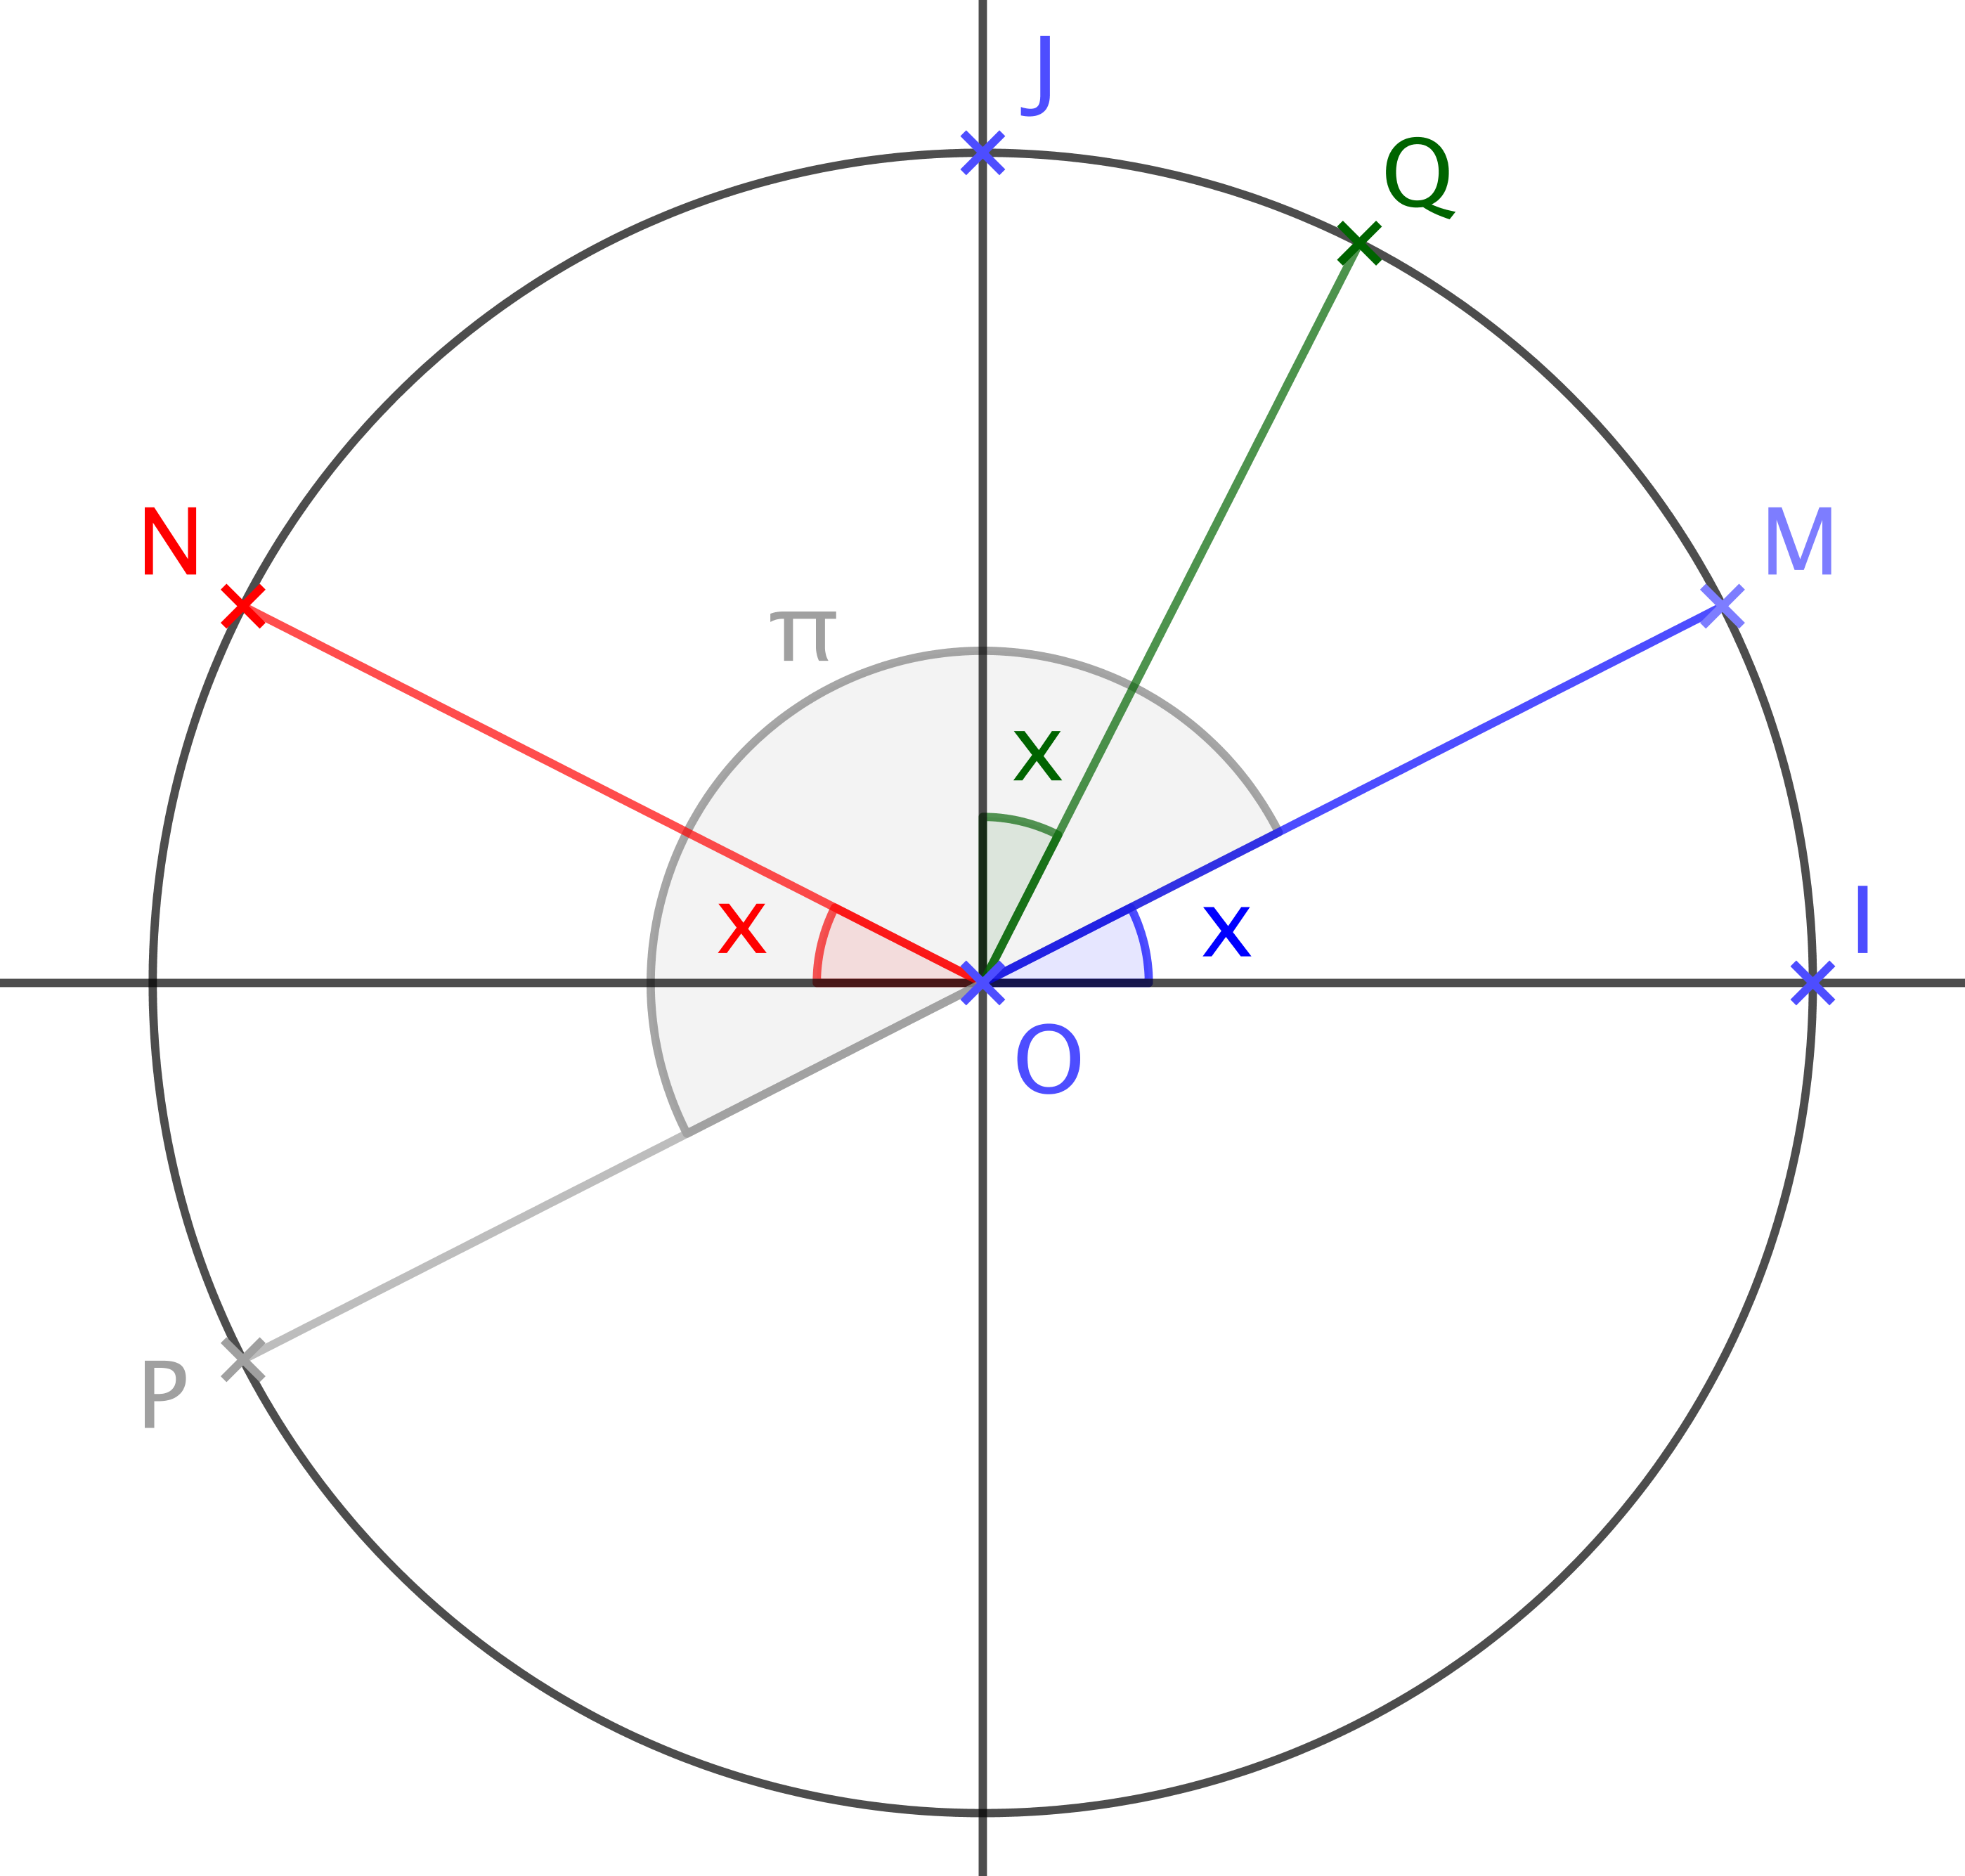
\includegraphics[scale = .7]{/trigo-identities/some-trig-formulas.png}}
	\end{center}
	\vspace{-3em}
\end{wrapfigure} 


A l'aide du dessin ci-contre, où les mesures des angles sont en radians, il est facile, via les points $M$ , $N$ , $P$ et $Q$ , de fournir des arguments géométriques justifiant que sous la condition $x\in \intervalO{0}{\frac{\pi}{4}}$ , on a :

\begin{itemize}[label=\small\textbullet]
	\item $\cos (\pi - x) = - \cos x$

	      \noindent
	      $\sin (\pi - x) = \sin x$ 

	\smallskip
	\item $\cos (x + \pi) = - \cos x$

	      \noindent
	      $\sin (x + \pi) = - \sin x$

	\smallskip
	\item $\cos \left( \frac{\pi}{2} - x \right) = \sin x$

	      \noindent
	      $\sin \left( \frac{\pi}{2} - x \right) = \cos x$ 
\end{itemize}


De nouveau, il serait bien de pouvoir passer à la validité des formules précédentes sur $\RR$ tout entier sans plus d'effort \emph{(considérer les autres cas n'est pas compliqué mais c'est un peu pénible)}.


\medskip

Nous allons voir que cela est licite grâce au fait \ref{holo-nullity} suivant qui est un peu technique car il nécessite la notion de fonction holomorphe que nous allons définir de suite.


\medskip

\begin{definition*}
	Soit une fonction complexe $f$ définie sur un ouvert $\Omega$ de $\CC$ .
	
	\smallskip
	
	$f$ est dite holomorphe en $\omega \in \Omega$ si la limite $\displaystyle \lim_{\stackrel{\abs{z - \omega} \, \rightarrow \, 0}{z \, \in \, \Omega - \geneset{\omega}}} \frac{f(z) - f(\omega)}{z - \omega}$ existe dans $\CC$ .
\end{definition*}


\medskip

Tout comme avec les fonctions réelles dérivables sur $\RR$, la propriété d'holomorphie se conserve par addition, multiplication, inverse et composition.


\medskip

\begin{fact} \label{holo-nullity}
	Soit $f$ une fonction holomorphe sur un ouvert $\Omega$ de $\CC$ . 
	
	\smallskip
	
	Si $\lambda \in \Omega$ vérifie $f(\lambda) = 0$ alors il existe un ouvert $V$ tel que $\lambda \in V \subseteq \Omega$ et $\forall z \in V - \geneset{\lambda}$ , $f(z) \neq 0$ 
	\emph{(c'est le prinicpe des zéros isolés d'une fonction holomorphe)}. 
\end{fact}


\begin{proof}
	Ceci nous amènerait trop loin donc nous admettrons ce résultat.
\end{proof}


\medskip

Pour conclure, il suffit de savoir que les fonctions circulaires réelles ne sont en fait que les restrictions à $\RR$ de fonctions holomorphes sur $\CC$ tout entier, et de noter que le raisonnement géométrique au début de cette section fait clairement apparaître des zéros non isolés pour les fonctions holomorphes sur $\CC$ ci-dessous
\footnote{
	Nous admettrons ces affirmations qui ne sont pas violentes à démontrer une fois que l'on a les bases de la théorie des fonctions holomorphes.
}.

\begin{itemize}[label=\small\textbullet]
	\item $A(z) = \cos (\pi - z) + \cos z$ 
	   et $B(z) =\sin (\pi - z) - \sin z$ 

	\smallskip
	\item $C(z) =\cos (z + \pi) + \cos z$ 
	   et $D(z) =\sin (z + \pi) + \sin z$

	\smallskip
	\item $E(z) =\cos \left( \frac{\pi}{2} - z \right) - \sin z$ 
	   et $F(z) =\sin \left( \frac{\pi}{2} - z \right) - \cos z$ 
\end{itemize}

